\chapter{平均场壳模型}

\section{价空间}
\begin{definition}[价空间(模型空间)]
    多核子组态中,由一些活跃的单粒子轨道组成的壳层结构。
\end{definition}
原子核价空间举例 如\Cref{fig:valence-space}所示:费米能级在幻数20的位置;低于费米能级的是$0\rm{d}-1\rm{s}$主壳的活跃空穴态(与空穴产生算符$h_{\beta}^{\dagger}$相关),高于费米能级的是$0\rm{f}-1\rm{p}-0\rm{g}_{9/2}$壳层(包含两个主壳,与粒子产生算符$c_{\alpha}^{\dagger}$相关);以上轨道的核子会从$0\rm{d}-1\rm{s}$跨过费米能级跃迁至$0\rm{f}-1\rm{p}-0\rm{g}_{9/2}$从而产生低激发能的跃迁。$0\rm{d}-1\rm{s}$主壳构成了粒子-空穴真空$\ket{\rm{HF}}$的填充部分,$0\rm{f}-1\rm{p}-0\rm{g}_{9/2}$则是$\ket{\rm{HF}}$的空轨道。
低于$0\rm{d}-1\rm{s}$壳层的所有轨道,也就是低于幻数8的所有单粒子轨道,一般认为具有惰性,即不活跃,这种不活跃的最低范围内的轨道称为\textcolor{red}{核心},核心是有效的粒子真空,满足
\begin{equation}
    \boxed{
    c_{\alpha} \ket{\rm{CORE}} = 0 \quad \text{for all $\alpha$ in valence space}
    }
\end{equation}
\begin{figure}[htbp]
    \centering
    \setlength{\abovecaptionskip}{0.2cm}
    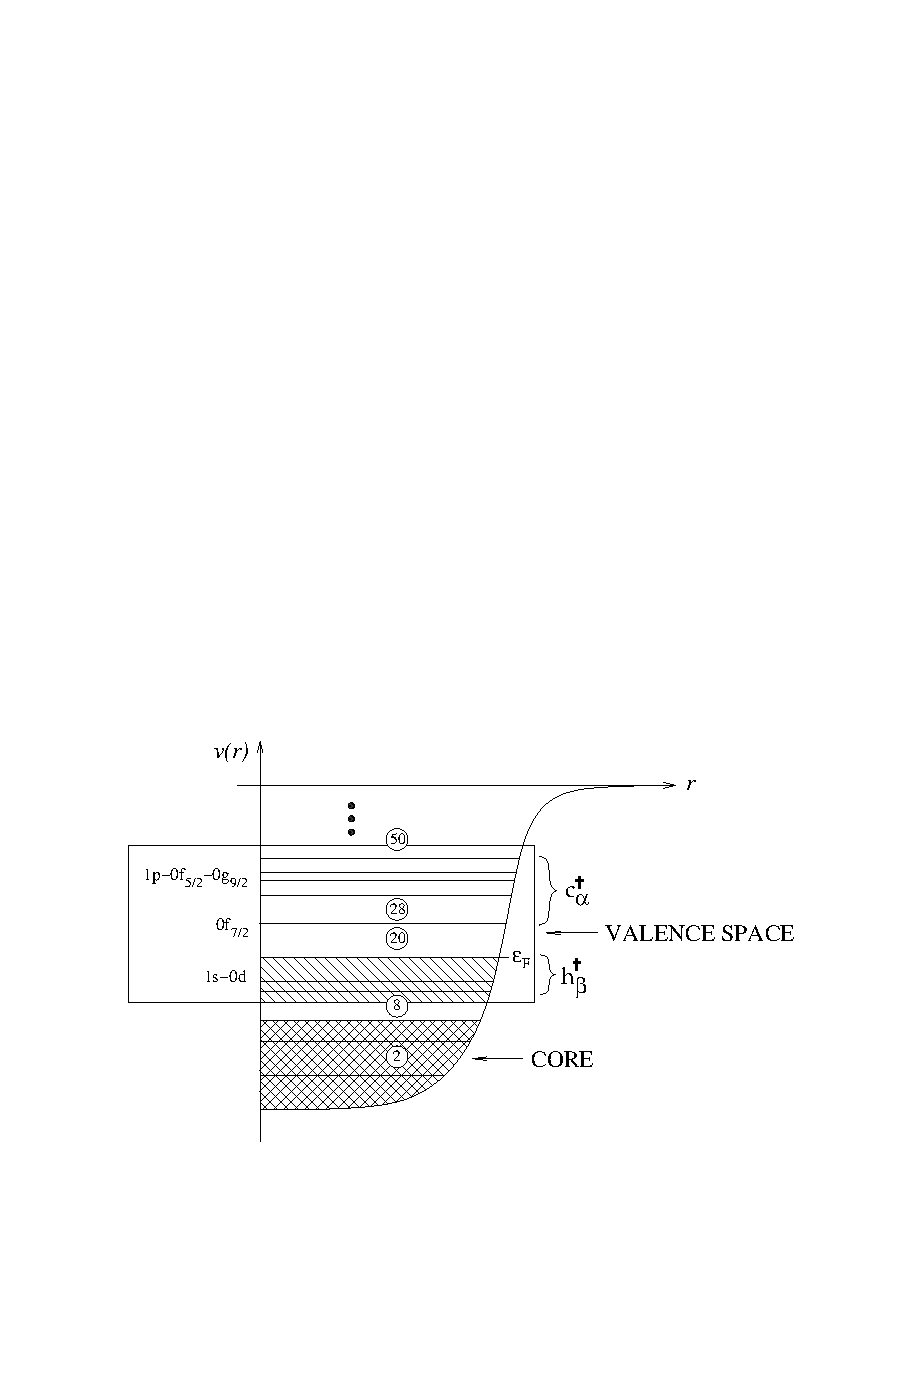
\includegraphics[scale=1.2]{figure/nuclear/valence-space.pdf}
    \caption{价空间与核心。}
    \label{fig:valence-space}
\end{figure}
价空间与核心的具体划分详见《\textit{From Nucleons to Nucleus Concepts of Microscopic Nuclear Theory}》中Sec. 5.1。

仅讨论如下原子核:
\begin{enumerate}
    \item 幻核(Magic nuclei):质子和中子都为幻数,填满主壳层的原子核。
    \item 半幻核(Semi-magic nuclei):中子(质子)为幻数,但质子(中子)不是幻数的原子核。
    \item 近幻核:拥有一个或两个价核子或价空穴的原子核。
\end{enumerate}


%%%%%%%%%%%%%%%%%%%%
\section{少核子系统的同位旋表示}
中子和质子一般认为是两种不同的粒子,在质子-中子表示中,用符号$\pi = (p, m_\pi)$和$\nu = (n, m_\nu)$分别对质子和中子进行标记。此外,我们也可用同位旋表示来标记质子和中子,同位旋标记中,质子和中子只是两个不同的同位旋态,取向上为中子态,向下为质子态\footnote{这种表示常见于核物理中,它使得大多数和具有正的总同位旋投影$M_{T} = \frac{1}{2}(N - Z)$。在粒子物理中一般取“同位旋向上”为质子,“同位旋向下”为中子。}:
\begin{equation}
    \boxed{
        \begin{aligned}
            \ket{n} =& \ket{t = \frac{1}{2}, m_{t} = +\frac{1}{2}} = \chi_{\frac{1}{2}, +\frac{1}{2}}^{T} = \begin{pmatrix}
                1 \\
                0
            \end{pmatrix} \\
            \ket{p} =& \ket{t = \frac{1}{2}, m_{t} = -\frac{1}{2}} = \chi_{\frac{1}{2}, -\frac{1}{2}}^{T} = \begin{pmatrix}
                0 \\
                1
            \end{pmatrix}
        \end{aligned}
    }
\end{equation}
上述两个核子态与粒子自旋态类似,可用类似泡利自旋矩阵联系起来。上式中,$t = \frac{1}{2}$是同位旋“长度”量子数,$m_{t}$是对应的投影。除了$\hbar$,同位旋$t = \frac{1}{2}$与自旋$s = \frac{1}{2}\hbar$完全类似。

类似角动量的定义,同位旋$\bmt$满足
\begin{equation}
    \boxed{
        t^{\dagger}_{k} = t_k, \quad k = 1, 2, 3,\quad \left[t_i, t_j\right] = \rm{i} \sum_{k}\epsilon_{ijk}t_{k}
    }
\end{equation}
按核子自旋的性质,同位旋同样有
\begin{align}
    \bmt^2 \ket{n} =& \frac{3}{4} \ket{n}, \quad t_3\ket{n} = +\frac{1}{2} \ket{n} \\
    \bmt^2 \ket{p} =& \frac{3}{4} \ket{p}, \quad t_3\ket{p} = -\frac{1}{2} \ket{p}
\end{align}
同样的,有


